\documentclass[11pt]{article}
\usepackage{amssymb}
\usepackage[english]{babel}
\usepackage{fullpage}
\usepackage{graphicx}
\graphicspath{ {./images/} }
\usepackage{spverbatim}


\def\titre{}
\def\auteur{}
\def\courriel{}



\makeatletter

\title{INF6306\\Patrons pour la compr\'{e}hension de programme}

\author{
    Foutse Khomh \\
    D\'{e}partement G\'{e}nie Informatique et G\'{e}nie Logiciel \\
    \'{E}cole Polytechnique de Montr\'{e}al, Qu\'{e}bec, Canada \\
    \texttt{foutse.khomh@polymtl.ca}
}

\date{}



\begin{document}
\maketitle

\section{Identification}

\paragraph{First, last name of the students:} Javier Rosales, Isabela Viera, Mahmood \auteur 
\paragraph{Date:} November 04, 2018.

\paragraph{Practice 1}\titre


\section{Practice 1}


\paragraph{Singleton:\\}

The following Singleton pattern was found in the following instance: 'w.tools.explorer.model.Attri-
buteModelBuilder::singleton:fw.tools.explorer.model.AttributeModelBuilder'

\begin{center}
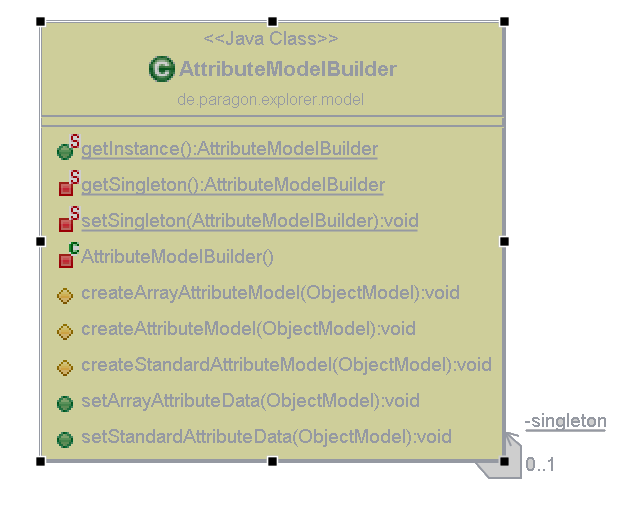
\includegraphics{Singleton}
\end{center}

The pattern involves a single class which create and object like while making sure that only single object is created.

In the next source code we can see its creating a single instance with the createAttributeModel function and its getting it in the AttributeModelBuilder:

\begin{spverbatim}
package de.paragon.explorer.model;

import java.lang.reflect.Field;
import java.util.Collections;
import java.util.Vector;

import de.paragon.explorer.util.StandardEnumeration;

public final class AttributeModelBuilder {
	private static AttributeModelBuilder	singleton;

	public static AttributeModelBuilder getInstance() {
		return AttributeModelBuilder.getSingleton();
	}

	private static AttributeModelBuilder getSingleton() {
		if (AttributeModelBuilder.singleton == null) {
			AttributeModelBuilder.setSingleton(new AttributeModelBuilder());
		}
		return AttributeModelBuilder.singleton;
	}

	private static void setSingleton(AttributeModelBuilder builder) {
		AttributeModelBuilder.singleton = builder;
	}

	private AttributeModelBuilder() {
		super();
	}

	protected void createArrayAttributeModel(ObjectModel objModl) {
		AttributeModel attrModl = new ArrayAttributeModel();
		objModl.addAttributeModel(attrModl);
		attrModl.setObjectModel(objModl);
	}

	/**
	 * Kommentar: Diese Methode geht davon aus, dass das ObjectModel bereits mit
	 * einem Object versehen ist. Fuer jedes Feld dieses Objects erzeugt sie ein
	 * neues AttributeModel und verknuepft es mit dem ObjectModel.
	 */
	protected void createAttributeModel(ObjectModel objModl) {
		AttributeModel attrModl = new AttributeModel();
		objModl.addAttributeModel(attrModl);
		attrModl.setObjectModel(objModl);
	}

	protected void createStandardAttributeModel(ObjectModel objModl) {
		AttributeModel attrModl = new StandardAttributeModel();
		objModl.addAttributeModel(attrModl);
		attrModl.setObjectModel(objModl);
	}

	/**
	 * Kommentar: Diese Methode geht davon aus, das bereits fuer jedes Feld des
	 * Objects in objectModel ein AttributeModel er- zeugt wurde. Jedem dieser
	 * AttributeModels wird der jeweilige Wert des Feldes zugewiesen.
	 */
	public void setArrayAttributeData(ObjectModel objModl) {
		int i = 0;
		// Object aObject;
		StandardEnumeration attrModls = objModl.getAttributeModels();
		while (attrModls.hasMoreElements()) {
			ArrayAttributeModel attrModl = (ArrayAttributeModel) attrModls.nextElement();
			// aObject = Array.get(objModl.getObject(), i);
			attrModl.setPos(i);
			attrModl.setName("[" + (Integer.valueOf(i)).toString() + "]");
			attrModl.setType(objModl.getObject().getClass().getComponentType());
			// if (aObject != null) {
			// attrModl.setValue(aObject);
			// } else {
			// attrModl.setValue(NullObject.getNullObject());
			// }
			i = i + 1;
		}
	}

	/**
	 * Kommentar: Diese Methode geht davon aus, das bereits fuer jedes Feld des
	 * Objects in objectModel ein AttributeModel erzeugt wurde. Jedem dieser
	 * AttributeModels wird der jeweilige Wert des Feldes zugewiesen.
	 */
	public void setStandardAttributeData(ObjectModel objModl) {
		int i = 0;
		// Object aObject;
		Field field;
		StandardEnumeration attrModls = objModl.getAttributeModels();
		Vector<Field> fields = objModl.getDeclaredFields();
		while (attrModls.hasMoreElements()) {
			StandardAttributeModel attrModl = (StandardAttributeModel) attrModls.nextElement();
			field = fields.elementAt(i);
			attrModl.setField(field);
			attrModl.setModifiers(field.getModifiers());
			attrModl.setType(field.getType());
			attrModl.setName(field.getName());
			i = i + 1;
		}
		Vector<AttributeModel> vector2set = new Vector<AttributeModel>();
		Vector<?> vector2transfer = attrModls.getVector();
		for (Object object2 : vector2transfer) {
			vector2set.add((AttributeModel) object2);
		}
		Vector<AttributeModel> vector = vector2set;
		Collections.sort(vector, new AttributeModelComparator());
	}
}


\end{spverbatim}


% Maximum one page!

\end{document}
